
\usepackage[T1]{fontenc}
\usepackage{mathptmx}
\usepackage[scaled=.90]{helvet}
\usepackage{courier}

\usepackage{beamerthemesplit}
\usepackage{verbatim}
\usepackage{hyperref}
\usepackage{listings}
\lstset{language=Perl,basicstyle=\footnotesize,tabsize=3,showstringspaces=false}

\setbeamerfont{single}{size=\huge}

\title{Modern PerlCommerce}
\author[racke]{Stefan Hornburg (Racke)\\ \texttt{racke@linuxia.de}}
\date[]{14th German Perl-Workshop, 28th February 2012, Erlangen}

\begin{document}
\maketitle{}

\begin{frame}
  \titlepage
\end{frame}

\tableofcontents

\section{Interchange}

\begin{frame}{Interchange}
\begin{itemize}
\item Around since 1995.
\item Fast and stable.
\item Flexible and extensible.
\end{itemize}
\end{frame}

\begin{frame}{Showcases}
\begin{itemize}
\item Backcountry \url{http://www.backcountry.com/}
\item FragnanceNet \url{http://www.fragrancenet.com/}
\end{itemize}
\end{frame}

As a single person, I'm involved in about 20 Interchange
projects in 6 countries. 80\% of my income comes from
these projects.

\begin{frame}{My projects}
\begin{itemize}
\item 20 projects
\item 6 countries
\item 80\% income
\end{itemize}
\end{frame}

\begin{frame}{Interchange}
\usebeamerfont{single}
\only{Sounds wonderful!}
\only<2>{}
\only<2>{Really?}
\end{frame}

% Interchange sites
% materialboerse.de (DE)
% passionshop.com (US)
% tj + cd (NL, FR)
% VSC, Training (AT)
% vinson/Webhostny (US)
% 2 * ulisses (DE)
% Linuxia, ICDEVGROUP (DE, US)
% SI 

\subsection{Caveats}

\begin{frame}{Community}
\begin{itemize}
\item Small group of developers
\item Little activity
\item Same people
\item Not part of CPAN
\end{itemize}
\end{frame}

Interchange is around since CGI.

\begin{frame}{Developer}
\begin{itemize}
\item Monolithic
\item Same codebase
\item Hard to find things
\end{itemize}
\end{frame}

\begin{frame}{User}
\begin{itemize}
\item Obscure templating
\item Missing extensions
\item Bad demo
\end{itemize}
\end{frame}

So I can still live with my current projects and even get
new projects through my existing customers, but it's next
to impossible to compete with other companies to get
new customers which don't know much about me.

This guy is solid, fast, but intimidating and
doesn't leave room for innovations.

\begin{frame}{Past}
  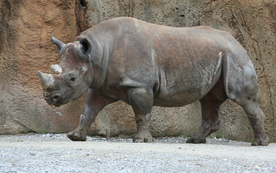
\includegraphics{rhino.jpg}
\end{frame}

\subsection{Alternatives}
Surprisingly there are not many choices for OpenSource PerlCommerce
software. Searching for ``cart'', ``ecommerce'' or ``shop'' on CPAN
gives you only a few results, which aren't actually very helpful.

Let's look at the possible choices for OpenSource PerlCommerce software:

\begin{frame}{Alternatives to Interchange}
\begin{itemize}
\item Handel
\item Agora
\item Business::Cart::Generic
\end{itemize}
\end{frame}

Handel is a framework which support AxKit, Template Toolkit 
and Catalyst.
Available from CPAN, last release a year ago.
There isn't even a mailing list.

Agora isn't modern Perl either and is around since 1999.

Business::Cart::Generic claims to be a basic shopping cart,
the synopsis says Convert parts of osCommerce and PrestaShop into
Perl.

\section{Future}
\subsection{We need a plan!}

\begin{frame}{Future}
\usebeamerfont{single}
\begin{itemize}
\item{Problem with Existing Codebase}
\item<2-3>{Missing alternatives}
\item<3>{Strong competitors}
\end{itemize}
\end{frame}

\begin{frame}{Future}
\usebeamerfont{single}
We need a plan!
\end{frame}

\begin{frame}{Future}
\usebeamerfont{single}
\begin{itemize}
\item Rewrite from scratch ?
\item<2-3> Too much work ?
\item<3> Modern Perl to the rescue!
\end{itemize}
\end{frame}

\subsection{Modern Perl}

\begin{frame}{Modern Perl}
\begin{itemize}
\item Plack/PSGI
\item OO
  \begin{itemize}
  \item Moose
  \item Moo
  \end{itemize}
\item Web Frameworks
 \begin{itemize}
  \item Dancer
  \item Catalyst
  \item Mojolicious
  \end{itemize}
\end{itemize}
\end{frame}

\subsubsection{Delegated Tasks}
By using an existing web framework which is Plack/PSGI compatible
we get relieved of the following
tasks and gain more flexibility in
addition.
 
\begin{frame}{Delegated Tasks}
\begin{itemize}
\item Dispatching requests
\item Parameter parsing
\item Session handling
\item Template engine
\end{itemize}
\end{frame}

\subsubsection{Extensions}
\begin{frame}{Extensions}
\begin{itemize}
\item Bundles
\item Plugins
\item Hooks
\end{itemize}
\end{frame}

\subsection{Policy}

\begin{frame}{Policy}
\begin{itemize}
\item KISS
\item Components
\item Assumptions
\item Expressive
\end{itemize}
\end{frame}

\begin{frame}{Future}
  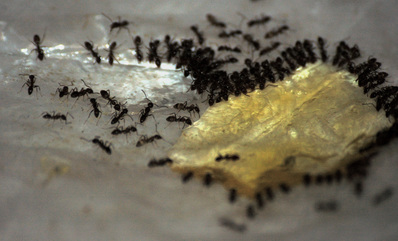
\includegraphics{ants.jpg}
\end{frame}

% \subsection{Modern Perl}
% There isn't really a set definition what Modern Perl is about,
% so I want to point the things important to us.

% \begin{frame}{Modern Perl - OO}
% \begin{itemize}
% \item Moose
% \item Mouse
% \item Moo
% \end{itemize}
% \end{frame}

% \begin{frame}{Modern Perl - Web Frameworks}
% \begin{itemize}
% \item Catalyst
% \item Dancer
% \item Mojolicious
% \end{itemize}
% \end{frame}

% \begin{frame}{Modern Perl - ORM}
% \begin{itemize}
% \item DBIx::Class
% \item Rose::DB
% \end{itemize}
% \end{frame}

% \section{Past and Future}

% \subsection{Past}
% \begin{frame}{Past}
% \begin{itemize}
% \item 1995 CGI
% \item 1995 MiniVend
% \item 1998 \url{http://www.materialboerse.de/}
% \item 2001 Interchange
% \end{itemize}
% \end{frame}


% % solid +
% % fast +
% % archaic -
% % monolithic -


While there are still a lot of sites with Interchange around,
there are basically no new projects done with Interchange.

\subsubsection{Principles}
Examples for being agnostic:

The Cart class doesn't make assumptions where the items are
stored, they could be in the session or in the database.

The Account Manager class allows multiple authentication
methods through account providers.

We don't have a fixed templating system like in Interchange.

We are not tied to a certain framework.

\begin{frame}{Assumptions}
Cart
\begin{itemize}
\item Session
\item DBI
\item Webservice *
\end{itemize}
\end{frame}

\begin{frame}{Assumptions}
Account Manager
\begin{itemize}
\item DBI
\item LDAP *
\item OpenID *
\end{itemize}
\end{frame}

\begin{frame}{Assumptions}
Templating Engine
\begin{itemize}
\item Template::Toolkit
\item Template::Flute
\end{itemize}
\end{frame}

\begin{frame}{Assumptions}
Web framework
\begin{itemize}
\item Catalyst
\item Dancer
\item Mojolicious
\end{itemize}
\end{frame}

To have these choices is good for developers and experienced users, 
but many users want to exactly know what they are getting.

Dancer fits our preferences the best.

Template::Flute allows us to use pure HTML templates.

DBI is the common storage method for Ecommerce products.

\begin{frame}{Preferences}
\begin{itemize}
\item Dancer
\item Template::Flute
\item DBI
\end{itemize}
\end{frame}

\subsubsection{Features}
\begin{frame}{Features}
\begin{itemize}
\item Navigation
\item Cart
\item Checkout
\item Accounts
\end{itemize}
\end{frame}

% \subsection{How easy can it be?}
% \begin{frame}[fragile]{How easy can it be?}
% \begin{lstlisting}
% #!/usr/bin/env perl

% use Dancer;
% use Dancer::Plugin::Interchange;

% sell;
% \end{lstlisting}
% \end{frame}

% \subsection{Real World}
% Running and maintaining an online shop is a challenging business
% and requires constant change to stay on top of your competitors.

% \begin{frame}{Real World}
% \begin{itemize}
% \item Marketing, SEO
% \item Legal stuff
% \item Interfaces
% \item Design
% \end{itemize}
% \end{frame}

\section{API}
\subsection{Cart}
\begin{frame}{Cart}
\begin{itemize}
\item SKU, Name, Quantity, Price
\item Price > 0
\item Combines automatically
\item Multiple carts
\item Storage everywhere
\item Price caching
\end{itemize}
\end{frame}

\begin{frame}[fragile]{Nitesi::Cart Methods}
\begin{lstlisting}
use Dancer::Plugin::Nitesi;

cart->add(sku => 'POM253', name => 'Pomelo',
    price => 3.00, quantity => 10);

cart->remove(sku => 'POM253');

cart->count();

cart->clear();

cart->total();

cart->subtotal();
\end{lstlisting}
\end{frame}

\subsubsection{Everything is a Cart}
\begin{frame}{Everything is a Cart}
\begin{itemize}
\item Saved Carts
\item Wishlists
\item Collections
\end{itemize}
\end{frame}

\begin{frame}[fragile]{Multiple Carts}
\begin{lstlisting}
cart('wishlist')->add(sku => 'ORA322', name => 'Orange',
     price => 2.00, quantity => 5);

\end{lstlisting}
\end{frame}

\subsubsection{Cart Backends}
\begin{frame}{Cart Backends}
\begin{itemize}
\item Session
\item DBI
\end{itemize}
\end{frame}

\subsubsection{Inventory Checks}
Inventory checks are pretty much limited in Interchange right now.
They are controlled by the configuration directives MinQuantityField
and MaxQuantityField:
\begin{frame}[fragile]{Inventory Check}
\begin{lstlisting}
MinQuantityField min_quantity
MaxQuantityField inventory:quantity 
\end{lstlisting}
\end{frame}
Also they are part of the standard code instead of loaded through
hooks.

\begin{frame}[fragile]{Inventory Check Hook}
\begin{lstlisting}
hook 'before_cart_add' => sub {
    my ($cart, $item) = @_;
    my ($inventory);

    $inventory = query->select_field(table => 'products',
                                     field => 'inventory',
                                     where => {sku => $item->{sku}});
				     
    if ($item->{quantity} > $inventory) {
        $item->{error} = 'Out of stock';
    }
};
\end{lstlisting}
\end{frame}

\subsubsection{Cart Hooks}
We just seen an example for before_cart_add hook.

The most common usage for after_cart_add is to update the cart
in the backend storage, for example storing the new item in the tables 
used by the DBI backend and update the modification date of the cart.

\begin{frame}{Cart Hooks}
\begin{itemize}
\item before\_cart\_add
\item after\_cart\_add
\item before\_cart\_update
\item after\_cart\_update
\item before\_cart\_remove
\item after\_cart\_remove
\end{itemize}
\end{frame}

after_cart_remove is used in a similar way as after_cart_add 
for removing the item in the tables used by the DBI backend
and update the modification date of the cart.

\subsection{Checkout}

\begin{frame}{Checkout}
\begin{itemize}
\item Taxes
\item Shipping
\item Payment
\item Invoice
\end{itemize}
\end{frame}

\subsubsection{Payment}
\begin{frame}{Payment}
\begin{itemize}
\item Business::CreditCard
\item Business::OnlinePayment
\end{itemize}
\end{frame}

\subsubsection{Taxes}
Tax on top of the product cost can be applied in different varieties.

Germany has 19\% salestax, 7.5\% reduced salestax for books and some
items are tax free. You have to show the breakdown of different taxes
on the receipt.

Orders for businesses between different countries of the EU are exempt
of salestax if the buying party has a salestaxid.

Business::Tax::VAT doesn't account for reduced rates.

\begin{frame}{Tax Modules on CPAN}
\begin{itemize}
\item Business::Tax::Canada
\item Business::CA::GST
\item Business::Tax::VAT
\item Business::Tax::VAT::Validation
\end{itemize}
\end{frame}

\subsubsection{Shipping}
\begin{frame}{Shipping}
\begin{itemize}
\item Simple Shipping
\item Crazy Shipping
\item Shipping API
\end{itemize}
\end{frame}

\subsubsection{Costs}
\begin{frame}{Costs}
\begin{itemize}
\item Tax
\item Shipping
\item Coupons
\end{itemize}
\end{frame}

\begin{frame}[fragile]{Absolute Costs}
\begin{lstlisting}
$cart->apply_cost(amount => 5, 
                  name => 'shipping', 
                  label => 'Shipping');
\end{lstlisting}
\end{frame}

\begin{frame}[fragile]{Relative Costs}
\begin{lstlisting}
$cart->apply_cost(amount => 0.19, 
                  relative => 1, 
                  name => 'tax', 
                  label => 'Salestax');
\end{lstlisting}
\end{frame}

\begin{frame}[fragile]{Inclusive Costs}
\begin{lstlisting}
$cart->apply_cost(amount => 0.19, 
                  relative => 1, 
                  inclusive => 1, 
                  name => 'tax', 
                  label => 'Salestax');
\end{lstlisting}
\end{frame}

\subsubsection{PDF Invoices}
\begin{frame}{PDF Invoices}
\begin{itemize}
\item HTML template
\item Template::Flute::PDF
\end{itemize}
\end{frame}

\subsection{Products}
\begin{frame}[fragile]{Product Class}
\begin{lstlisting}
package Nitesi::Product;

use Moo;

has sku => (is => 'rw');
has name => (is => 'rw');
has description => (is => 'rw'); 
has price => (is => 'rw');
has weight => (is => 'rw');
has priority => (is => 'rw');
has inactive => (is => 'rw');

1;
\end{lstlisting}
\end{frame}

\begin{frame}[fragile]{Product Subclass}
\begin{lstlisting}
package MyShop::Product;

use Moo;
use base 'Nitesi::Product';

has inventory (is => 'rw');

1;
\end{lstlisting}
\end{frame}

\begin{frame}[fragile]{Product Backend}
\begin{lstlisting}
package Nitesi::Product::Backend::DBI;
use Moo;

has dbh => (is => 'rw');

has query => (
    is => 'ro',
    lazy => 1,
    default => sub {Nitesi::Query::DBI->new(dbh => shift->dbh);}
    );

sub load { ... };

sub save { ... };

1;
\end{lstlisting}
\end{frame}

\subsection{Accounts and Access Control}

\begin{frame}[fragile]{Accounts}
\begin{lstlisting}
post '/login' => sub {
    if (account->login(username => params('body')->{username},
                       password => params('body')->{password})) {
        redirect '/customerservice';
    }
    else {
        redirect '/login';
    }
};
\end{lstlisting}
\end{frame}

\begin{frame}[fragile]{Accounts}
\begin{lstlisting}
get '/mywishlist' => sub {
    if (account->acl(check => 'create_wishlists')) {
        return template 'mywishlist';
    }

    account->status(login_info => 'Please login to view wishlist.',
                    login_continue => 'mywishlist',
                   )

    redirect '/login';
};
\end{lstlisting}
\end{frame}

\subsubsection{Account Manager}
\begin{frame}{Account manager}
\begin{itemize}
\item Account Providers
\item Login/Logout
\item Account Information
\item Login status
\item Forgot password
\item Registration
\end{itemize}
\end{frame}

\subsubsection{Account Provider}
\begin{frame}{Account Provider}
\begin{itemize}
\item DBI 
\item LDAP *
\item Htpasswd * 
\item OpenID *
\item OAuth *
\end{itemize}
\end{frame}

\subsubsection{Access Control}
\begin{frame}{Access Control}
\begin{itemize}
\item User
\item Roles
\item Permissions
\end{itemize}
\end{frame}

\subsection{Forms}
\begin{frame}{Forms}
\begin{itemize}
\item Display
\item Validation
\item Storage
\end{itemize}
\end{frame}

\subsection{Web Services}
\begin{frame}{Web Services}
\begin{itemize}
\item REST
\item XML-RPC
\item SOAP
\end{itemize}
\end{frame}

\section{Development}

\begin{frame}{Nitesi}
  
\includegraphics{nitesi.png}
\end{frame}

\subsection{Projects}
\subsubsection{Vienna Shopping Cart}
\begin{frame}{Vienna Shopping Cart}
\url{https://vsc.state.gov/}
\end{frame}

\subsubsection{Payment Gateway}
\begin{frame}{Payment Gateway}
  \begin{itemize}
  \item charge keyword
  \item Business::OnlinePayment
  \item ACI payment system
  \end{itemize}
\end{frame}

\subsubsection{OpenERP Interface}
\begin{frame}{OpenERP Interface} 
  \begin{itemize}
  \item XML-RPC
  \end{itemize}
\end{frame}

\subsubsection{Backend/CRM}
\begin{frame}{Backend/CRM} 
  \begin{itemize}
  \item Backend
  \item CRM
  \end{itemize}
\end{frame}

\subsubsection{Demo Shop}
\begin{frame}{Demo Shop} 
  \begin{itemize}
  \item Templates
  \item Navigation
  \item Database
  \item Payment Tests
  \end{itemize}
\end{frame}

\subsection{Contribution}
\subsubsection{Nitesi @ CPAN/GitHub}
\begin{frame}{CPAN/GitHub}
\begin{itemize}
\item \url{https://metacpan.org/module/Nitesi}
\item \url{https://metacpan.org/module/Nitesi::DBI/}
\item \url{https://metacpan.org/module/Dancer::Plugin::Nitesi/}
\end{itemize}
\begin{itemize}
\item \url{https://github.com/racke/Nitesi}
\item \url{https://github.com/racke/Nitesi-DBI}
\item \url{https://github.com/racke/Dancer-Plugin-Nitesi}
\end{itemize}
\end{frame}

\subsection{Slides and Contact}
\begin{frame}{Slides and Contact}
Slides:
\begin{itemize}
\item \url{http://www.linuxia.de/talks/perlcommerce/perlcommerce-beamer.pdf}
\item \url{http://conferences.yapceurope.org/gpw2012/schedule}
\end{itemize}

Email:
\begin{itemize}
\item racke@linuxia.de
\end{itemize}

IRC:
\begin{itemize}
\item \#interchange irc.freenode.net
\item \#dancer irc.perl.org
\end{itemize}

\end{frame}

\subsection{Questions}
\begin{frame}{Questions}
\usebeamerfont{single}
\begin{itemize}
\item<1> Question !
\item<2> Questions ?
\end{itemize}
\end{frame}

\subsection{The End}
\begin{frame}{The End}
\usebeamerfont{single}
Thanks a lot!
\end{frame}

\end{document}

%%% Local Variables: 
%%% mode: latex
%%% TeX-master: t
%%% End: 
